%% LyX 2.2.3 created this file.  For more info, see http://www.lyx.org/.
%% Do not edit unless you really know what you are doing.
\documentclass[spanish]{article}
\usepackage[T1]{fontenc}
\usepackage[latin9]{luainputenc}
\usepackage{geometry}
\geometry{verbose,tmargin=2cm,bmargin=2cm,lmargin=2cm,rmargin=2cm,headheight=2cm,headsep=2cm}
\setlength{\parindent}{0bp}
\usepackage{graphicx}
\usepackage{babel}
\addto\shorthandsspanish{\spanishdeactivate{~<>}}

\begin{document}

\part{Oscilador de Wien}

\section{Introducci�n}

A lo largo de esta parte, se centrar� en realizar un oscilador generador
de onda sinusoidal basado en el puente de \emph{Wien.} Para poder
entender este oscilador, resulta necesario comprender el criterio
de Barkhausen, el cual es imprecindible para realizar el oscilador.

\subsection{Criterio de Barkhausen}

Dado un sistema realimentado negativamente, siendo \emph{A }la ganancia
de lazo abierto y $\beta$ la ganancia de realimentaci�n, entonces
se define $T(s)=A(s)\beta(s)$ como la ganancia de lazo de realimentaci�n.

\begin{figure}[h]
\begin{centering}
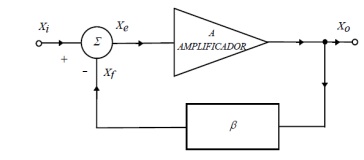
\includegraphics{Resources/Realimentado}
\par\end{centering}
\caption{Sistema realimentado}

\end{figure}

De acuerdo con lo desarrollado en el libro \emph{Design With Operational
Amplifiers And Analog Integrated Circuits}\footnote{\emph{A lo largo del capitulo 10.1 durante el desarrolo de Basic Wien-Bridge
Oscillator}}\emph{, }pueden ocurrir 3 posibles situaci�nes para la ganancia de
lazo de realimentaci�n \emph{T(s)}:
\begin{enumerate}
\item \emph{T($S_{0}$) < 1} : Lo cual supone una atenuaci�n de la se�al
por lo que el sistema resulta estable sin oscilar.
\item \emph{T($S_{0}$) > 1} : Lo cual genera una amplificaci�n de la se�al
resultando en un sistema inestable que con el correr del tiempo generar�
que el amplificador oscile
\item \emph{T($S_{0}$) = 1} : Esta es considerada una estabilidad neutral
ya que no atenua ni amplifica la se�al. Esta es la condici�n que se
tiene en cuenta para que el criterio funcione.
\end{enumerate}
De acuerdo con lo mencionado en el libro, para que se cumpla la condici�n
3, es necesario tener un par de polos conjugados sobre el eje $j\omega$.

\subsection{Oscilador de \emph{Wien}}

Dado un circuito como el que se muestra en la Figura \ref{1_1}, se
podr� calcular como se mencion� previamente, la ganancia de lazo de
realimentaci�n. 

\begin{figure}[h]
\begin{centering}
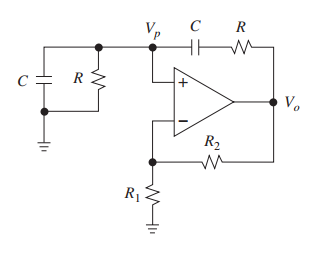
\includegraphics{Resources/CircuitoWien.PNG}
\par\end{centering}
\caption{Circuito de Wien}
\label{1_1}

\end{figure}

Como se menciona en el libro\footnote{Partiendo de la ecuaci�n 10.4 y 10.5 de la pagina 486 del libro}
se llega a la ecuaci�n mencionada a continuaci�n:

\begin{equation}
T(f)=\frac{1+\frac{R_{2}}{R_{1}}}{3+j\left(\frac{f}{f_{0}}-\frac{f_{0}}{f}\right)}\label{eq:1_1}
\end{equation}

\[
f_{0}=\frac{1}{2\pi RC}
\]

Por lo tanto, si se remplaza \emph{f} por la frecuencia $f_{0}$,
se obtiene

\begin{equation}
T\left(f_{0}\right)=\frac{1+\frac{R_{2}}{R_{1}}}{3}\label{eq:1_2}
\end{equation}

Consecuentemente, como se desea cumplir con la condici�n 3 mencionada
en la sbsecci�n anterior, necesariamente $\frac{R_{2}}{R_{1}}=2$.
Por ende, cuando se cumpla esta condici�n, resulta evidente que se
generar� un puente balanceado a lo largo de la frecuencia $f_{0}$.

\section{An�lisis del circuito propuesto}

A lo largo de esta secci�n nos centraremos en analizar el circuito
propuesto por la c�tedra que se puede observar en la Figura \ref{1_3}.

\begin{figure}[h]
\begin{centering}
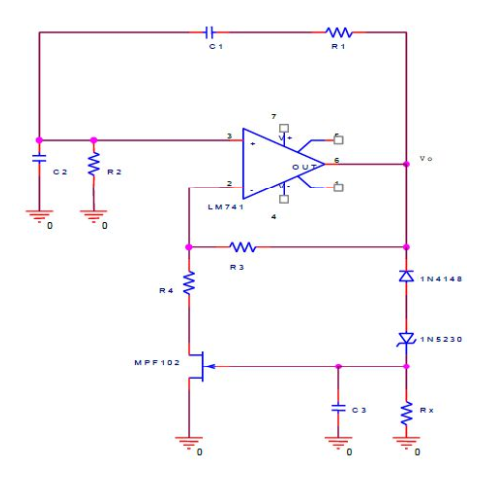
\includegraphics[scale=0.5]{Resources/Circuito}
\par\end{centering}
\caption{Circuito de Oscilador propuesto}
\label{1_3}

\end{figure}

Como se puede ver en la figura, el circuito propuesto es bastante
parecido al mencionado en la Figura \ref{1_1}, los componentes adicionales
agregados forman parte de lo que se llama \emph{Automatic Amplitude
Control}\footnote{Control Autom�tico de Ganancia o CAG en espa�ol}
(AAC). El AAC, es la etapa del circuito encargada de ajustar el valor
de $\frac{R_{3}}{R_{4}}$ din�micamente con el objetivo de suplir
las falencias constructivas de los elementos resistivos, que generan
un determinado error en el cociente, para llevarlo al valor esperado
de 2.

\subsection{\emph{Automatic Amplitude Control (AAC)}}

\subsubsection{Transistor JFET-N}

Para poder entender el funcionamiento del AAC, es necesario primero
entender como se comporta un JFET-N, para eso, se puede observar la
Figura \ref{1_4}.

\begin{figure}[h]
\begin{centering}
\includegraphics[scale=0.5]{\string"Resources/ids VS vds\string".png}
\par\end{centering}
\caption{$I_{DS}$ en funci�n de $V_{DS}$, para valores de VGS entre -3 (V)
(linea negra) y 0.5(V) (linea azul) }
\label{1_4}

\end{figure}

\begin{figure}[h]
\begin{centering}
\includegraphics[scale=0.4]{\string"Resources/RDS vs VDS 1\string".png}\includegraphics[scale=0.4]{\string"Resources/RDS vs VDS 2\string".png}
\par\end{centering}
\caption{$R_{DS}$en funci�n de $V_{DS}$ para valores de $V_{GS}$ entre -2.5(V)
(linea negra) y 0.5(V) (linea verde)}
\label{1_5}

\end{figure}

Como se pudo observar en la Figura \ref{1_5}, se pude utilizar al
transisto JFET-N como resistencia variable, esto es altamente �til
para ajustar el valor del cociente $\frac{R_{3}}{R_{4}}$ visto anteriormente
y utilizarlo a nuestro favor.

\subsubsection{Diodos en serie}

Debido a que el oscilador de wien debe poder funcionar sin se�al de
entrada, se debe crear un control sobre $\frac{R_{3}}{R_{4}}$ de
modo tal que, cuando el circuito se alimente, rapidamente se llegue
a la oscilaci�n. Esto se realiza mediante el cambo dinamico de $R_{4}$,
es decir, cuando el circuito permanezca apagado, y durante los primeros
instantes de alimentaci�n, $R_{4}$ debe permanecer lo suficientemente
baja poara que el cociente sea lo suficientemente mayor a 2 para lograr
un tiempo de establecimiento relativamente corto, sin embargo, una
vez que se llega a ese tiempo de establecimiento, se debe procurar
de aumentar el valor de $R_{4}$ de modo tal que el cociente de resistencias
sea 2, como fue explicado anteriormente. Para lograr esto, entran
en juego los diodos, que cuando la tensi�n Vo es lo suficientemente
chica, los diodos no conduzcan, generando asi que el JFET tenga una
resistencia interna aproximadamente igual a 0, y cuando Vo supera
la tensi�n de umbral de los diodos (aproximadamente 5.4(V)), estos
conduzcan corriente, cargen el capacitor C3 y ajusten la resistencia
interna del transistor $R_{T}$ para que $\frac{R_{3}}{R_{4}+R_{T}}<2$
\end{document}
